\documentclass[12pt,a4paper]{article}

% ---- Język i kodowanie ----
\usepackage{iftex}
\ifPDFTeX
  \usepackage[utf8]{inputenc}
  \usepackage[T1]{fontenc}
  \usepackage{lmodern}
\else
  \usepackage{fontspec}
\fi
\usepackage[polish]{babel}
\usepackage{indentfirst}

% ---- Układ strony ----
\usepackage{geometry}
\geometry{margin=2.5cm}
\usepackage{microtype}
\setlength{\parskip}{0.4em}

% ---- Tabele, listy, obrazy ----
\usepackage{float}
\usepackage{caption}
\captionsetup{font=small,labelfont=bf}
\usepackage{booktabs}
\usepackage{tabularx}
\usepackage{array}
\usepackage{enumitem}
\setlist{nosep,leftmargin=1.4em}
\newcolumntype{Y}{>{\raggedright\arraybackslash}X}
\usepackage{graphicx}

% ---- Kolory (spójne z dokumentem wizji) ----
\usepackage{xcolor}
\definecolor{gold}{HTML}{8A6D3B}
\definecolor{darkgold}{HTML}{5A4A2A}
\newcommand{\code}[1]{\texttt{\detokenize{#1}}}
\newcommand{\fig}[3]{%
\begin{figure}[H]\centering
\includegraphics[width=#2\textwidth]{#1}
\caption{#3}
\end{figure}}

% ---- Tytuły sekcji ----
\usepackage{titlesec}
\titleformat{\section}{\Large\bfseries\color{darkgold}}{\thesection}{0.6em}{}
\titleformat{\subsection}{\large\bfseries\color{gold}}{\thesubsection}{0.6em}{}

% ---- Hiperłącza ----
\usepackage[hidelinks]{hyperref}
\hypersetup{colorlinks=true,linkcolor=darkgold,urlcolor=gold}

\title{
    \large Projekt kompetencyjny IOAD 2026/2027 \\[0.3em]
    \Huge \textbf{Raport z prac} \\[0.3em]
    \LARGE PlayLink Multi-Region \\
    \large \textit{Co zostało zrobione (wersja na 18.11.2026)}
}
\author{
    Bartosz Kołaciński, nr indeksu: 251554 \\
    Mateusz Kosowski, nr indeksu: 251558 \\
    Nikodem Nowak, nr indeksu: 251598 \\
    Natan Ręklewski, nr indeksu: 252952 \\
    Jakub Rosiak, nr indeksu: 251620 \\
    Andrzej Krysiak, nr indeksu: 252945 \\[0.6em]
    \normalsize Opiekun projektu: mgr inż. Bartłomiej Jencz
}
\date{18 listopada 2026}

\begin{document}
\pagenumbering{gobble}
\maketitle
\vfill
\begin{center}
\small
Repozytorium: \url{https://github.com/ioad-modul-sumatywny-26/playlink}
\end{center}

\newpage
\pagenumbering{Roman}
\tableofcontents
\newpage
\pagenumbering{arabic}

% =====================================================================
\section{Cel i zakres raportu}
Raport opisuje, co zespół zbudował w projekcie \textbf{PlayLink Multi-Region}: aplikację do szukania
graczy (LFG) uruchomioną w dwóch regionach (EU i US) na Azure, razem ze sposobem wybierania regionu,
powtarzalnym wdrożeniem, eksperymentem obciążeniowym, logami z metrykami i serwerem MCP dla asystentów AI.
Opisane są tylko rzeczy faktycznie wykonane i sprawdzone: jak działają, jak je uruchomić, wraz ze
zrzutami ekranu, diagramami i listą zrealizowanych zadań. Układ odpowiada filarom F1--F7 z dokumentu wizji
(\code{docs/dokument-wizji.tex}).

% =====================================================================
\section{Co powstało w skrócie}
\begin{table}[H]
\centering\footnotesize
\renewcommand{\arraystretch}{1.25}
\begin{tabularx}{\textwidth}{@{}l>{\raggedright\arraybackslash}p{0.2\textwidth}Y@{}}
\toprule
\textbf{Filar} & \textbf{Temat} & \textbf{Co działa} \\
\midrule
F1 & Dwa regiony z lobby & Dwa niezależne stosy (EU, US) na Azure za Cloudflare Tunnel; \code{/healthz} obu regionów zwraca wersję \code{v0.2.0-rc.2} \\
F2 & Wybór regionu & Sonda opóźnień, cookie regionu, baner Stay/Switch, automatyczny failover (rys.~\ref{fig:chooser}) \\
F3 & Powtarzalne wdrożenie & \code{deploy/deploy.sh}, \code{deploy/azure-vm.sh}, wydania GHCR, aktualizacja pull-based; wydanie rc.2 wdrożone na EU i US \\
F4 & Eksperyment 1 vs 2 regiony & Runner w \code{experiments/f4/} z raportami JSON i Markdown; przebieg lokalny (rozdz.~\ref{sec:f4}) \\
F7 & Obserwowalność i MCP & Grafana z logami i metrykami obu regionów, serwer MCP z narzędziami do pokoi, logów i metryk \\
\bottomrule
\end{tabularx}
\caption{Zrealizowane filary projektu.}
\end{table}

% =====================================================================
\section{Co zostało zrobione}

\subsection{F1: dwa regiony z działającymi lobby}
Każdy region to osobna maszyna wirtualna z własną bazą PostgreSQL, backendem FastAPI i frontendem
SvelteKit (kontenery \code{db}, \code{backend}, \code{frontend}, \code{cloudflared}). Pokoje i czat są
\emph{regionalne}, tożsamość jest wspólna (klucz z frazy BIP39 zostaje w przeglądarce). Maszyny nie mają
otwartych portów publicznych: cały ruch wchodzi tunelem Cloudflare.

\fig{../diagrams/architektura-regionow.png}{1.0}{Architektura dwuregionowa: gracz, Cloudflare, maszyny EU, US i ops.}

Rysunki~\ref{fig:eu} i~\ref{fig:us} pokazują tę samą aplikację w obu regionach (lokalny odpowiednik stosu).
Region EU stoi w Polsce (\code{polandcentral}), region „US'' w Danii (\code{denmarkeast}), bo Azure for Students
nie udostępnia regionów w USA; mechanizm jest identyczny.

\begin{figure}[H]\centering
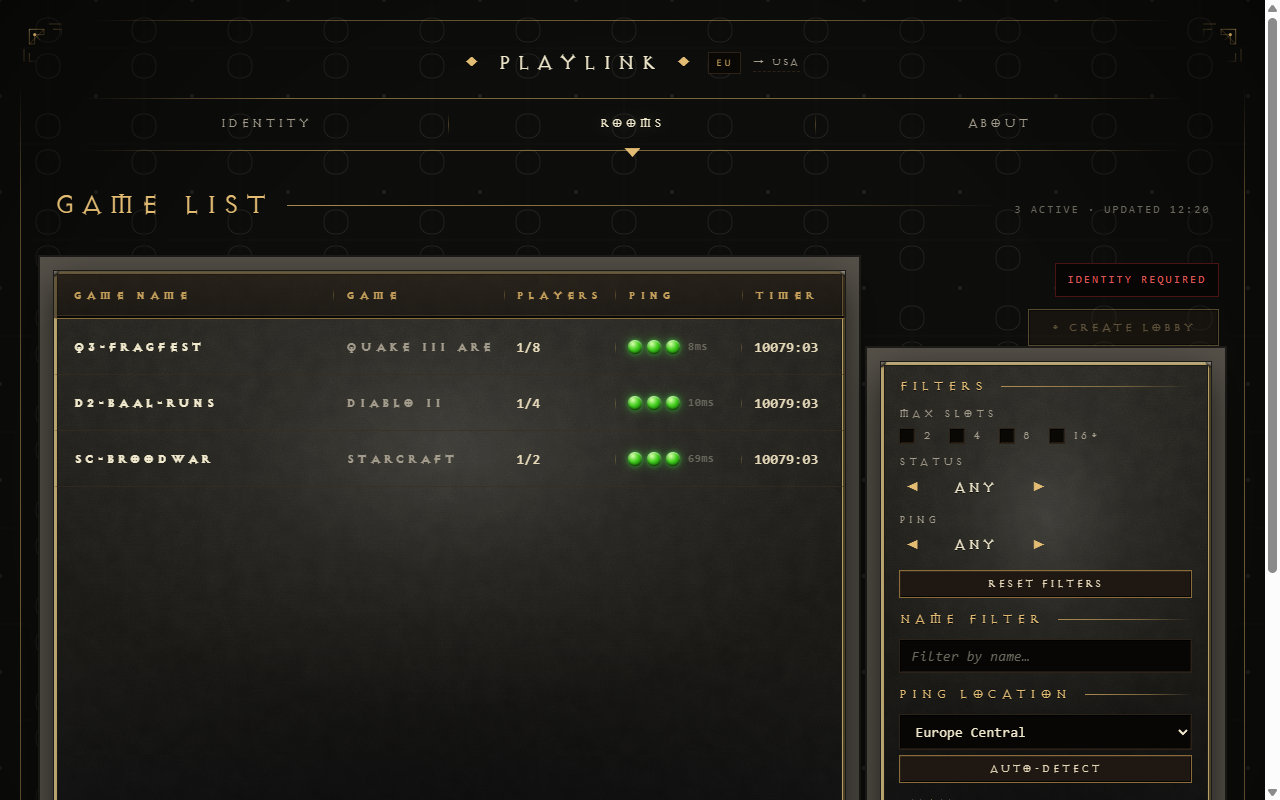
\includegraphics[width=0.8\textwidth]{obrazy/02-lobby-eu.png}
\caption{Lista pokoi w regionie EU.}\label{fig:eu}
\end{figure}
\begin{figure}[H]\centering
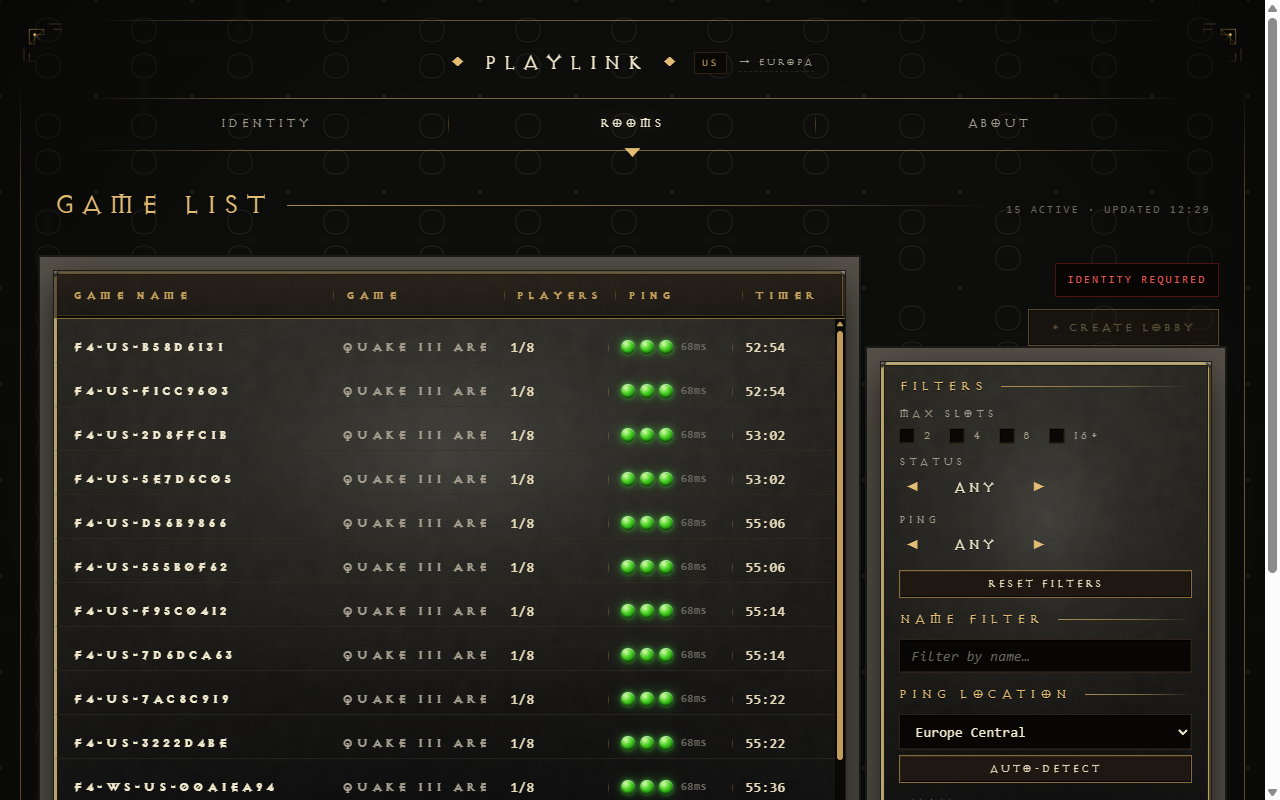
\includegraphics[width=0.8\textwidth]{obrazy/03-lobby-us.png}
\caption{Lista pokoi w regionie US (pokoje utworzone przez eksperyment F4).}\label{fig:us}
\end{figure}

\subsection{F2: wybór regionu}
Przy pierwszym wejściu przeglądarka mierzy czas odpowiedzi \code{/healthz} obu regionów i otwiera lobby
w szybszym. Wybór jest zapamiętany w cookie \code{playlink.region}. Szybszy drugi region jest tylko
\emph{propozycją} (baner Stay/Switch), a automatyczny failover następuje wyłącznie wtedy, gdy zapisany region
nie odpowiada. Ręczny przełącznik jest zawsze dostępny. Dodatkowo czat i lista pokoi używają heartbeatu
WebSocket (30~s) i automatycznie łączą się ponownie po zerwaniu połączenia.

\fig{../diagrams/wybor-regionu.png}{0.75}{Przebieg wyboru regionu: sonda, zapis, propozycja i failover.}

\begin{figure}[H]\centering
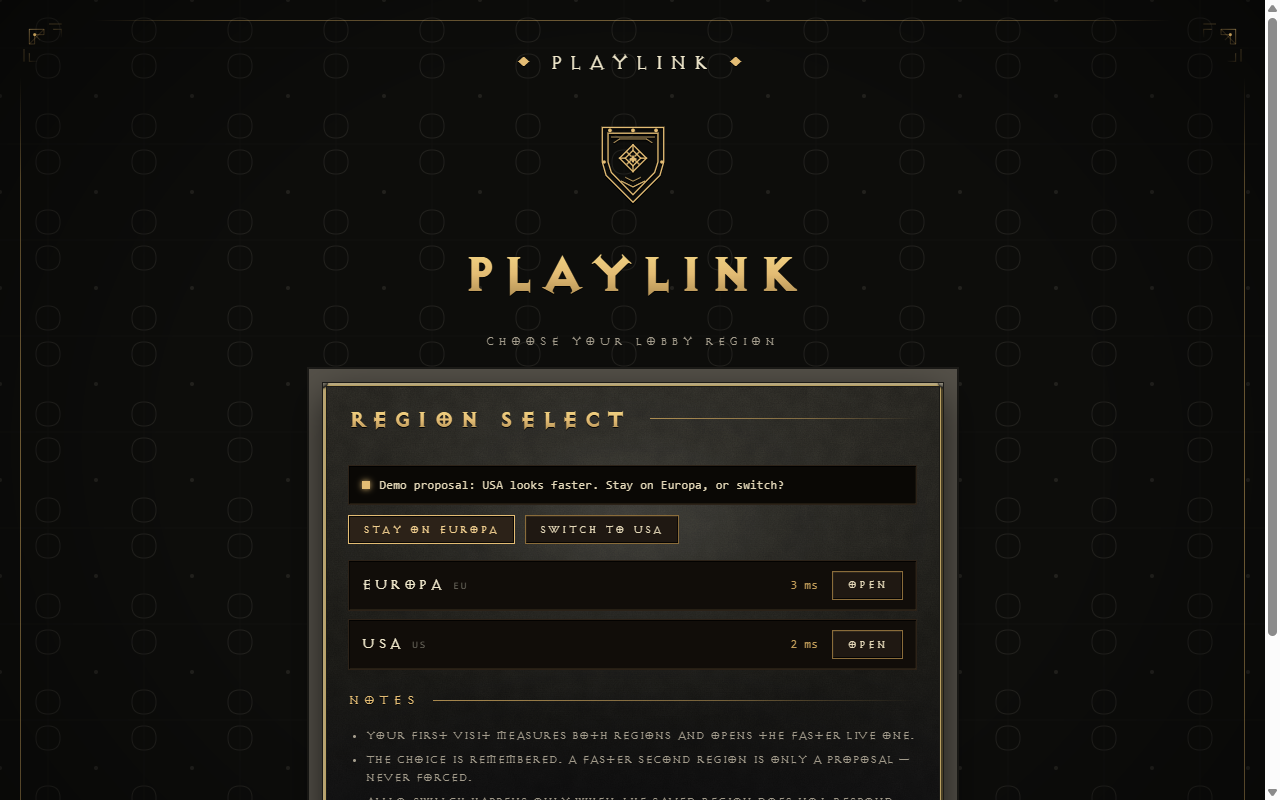
\includegraphics[width=0.85\textwidth]{obrazy/01-chooser.png}
\caption{Ekran wyboru regionu z propozycją zmiany (tryb demonstracyjny \code{?propose=1}).}\label{fig:chooser}
\end{figure}

\subsection{F3: powtarzalne wdrożenie}
Jedno polecenie (\code{deploy/deploy.sh <eu|us> [tag]}) stawia region lokalnie lub na maszynie, a
\code{deploy/azure-vm.sh} tworzy całą maszynę na Azure bez otwartych portów. Wydania budują się po wypchnięciu
tagu (\code{.github/workflows/release.yml}): testy, lint, migracje, obrazy w GHCR. Maszyny same pobierają
nową wersję co 2 minuty; US czeka, aż EU zgłosi nową wersję w \code{/healthz}, a zły release zatrzymuje się
na EU i jest cofany.

\fig{../diagrams/wdrozenie-pull.png}{0.8}{Wydanie i wdrożenie pull-based.}

W praktyce: 3.11.2026 wydano \code{v0.2.0-rc.2} (kod z PR 91--102) i wdrożono je na EU, a następnie na US.
Sprawdzono wersję w \code{/healthz} obu regionów.

\subsection{F4: eksperyment 1 vs 2 regiony}\label{sec:f4}
Runner \code{experiments/f4/run.py} porównuje wariant A (cały ruch na EU) z wariantem B (użytkownicy na przemian
EU i US) w scenariuszach: autoryzacja, lista pokoi, tworzenie, dołączanie, opuszczanie, czat WebSocket i
aktualizacja listy. Poniżej wynik przebiegu lokalnego (4 użytkowników, 3 iteracje, dwa stosy na jednej
maszynie z podniesionymi limitami żądań).

\begin{table}[H]
\centering\footnotesize
\begin{tabular}{@{}lrrr@{}}
\toprule
\textbf{Scenariusz} & \textbf{A p95 [ms]} & \textbf{B p95 [ms]} & \textbf{Różnica B--A} \\
\midrule
GET /rooms & 24,9 & 18,6 & $-6{,}2$ \\
POST /rooms & 80,6 & 58,8 & $-21{,}8$ \\
POST /rooms/\{name\}/join & 56,8 & 49,9 & $-6{,}9$ \\
POST /rooms/\{name\}/leave & 66,0 & 49,9 & $-16{,}1$ \\
Czat WebSocket (round-trip) & 56,3 & 24,9 & $-31{,}3$ \\
Aktualizacja listy (WS) & 28,0 & 30,0 & $+2{,}0$ \\
Autoryzacja (nonce + podpis) & 135,9 & 113,9 & $-22{,}1$ \\
\midrule
\textbf{Ogółem} & \textbf{119,6} & \textbf{97,1} & \\
\bottomrule
\end{tabular}
\caption{Wynik lokalny: 91 próbek w A i 106 w B, 0\% błędów. Wariant B jest szybszy tylko dlatego, że ruch
dzieli się między dwa backendy na jednej maszynie.}
\end{table}

Runner działa na dowolnych adresach, więc ten sam eksperyment można uruchomić na regionach publicznych:
\code{python run.py --variant both --eu <adres EU> --us <adres US>}. Przebieg lokalny potwierdza, że
metoda działa end-to-end (autoryzacja podpisem, REST, WebSocket) i daje powtarzalny raport. Scenariusze
awarii regionu (zatrzymanie backendu, tunelu lub bazy) są opisane w \code{docs/operations/runbook-regions.md}.

\subsection{F7: logi i metryki (Grafana)}
Każdy region ma dwa dodatkowe kontenery: Vector (wysyła logi kontenerów i metryki maszyny) i cAdvisor (metryki
każdego kontenera). Dane trafiają do osobnej maszyny \code{playlink-ops}: VictoriaLogs (logi, LogsQL),
VictoriaMetrics (metryki, PromQL) i Grafana z dashboardem „PlayLink regions''. Backend loguje JSON z
identyfikatorem żądania i zdarzeniami biznesowymi (logowanie, tworzenie i dołączanie do pokoi) oraz wystawia
\code{/metrics}; błędy frontendu (serwerowe i z przeglądarki) trafiają do tych samych logów. Grafana jest
chroniona Cloudflare Access (logowanie jednorazowym kodem z e-maila), a agenty w regionach tylko wysyłają dane,
więc regiony nadal nie mają otwartych portów.

\fig{../diagrams/obserwowalnosc.png}{1.0}{Przepływ logów i metryk od regionów do Grafany.}

\begin{figure}[H]\centering
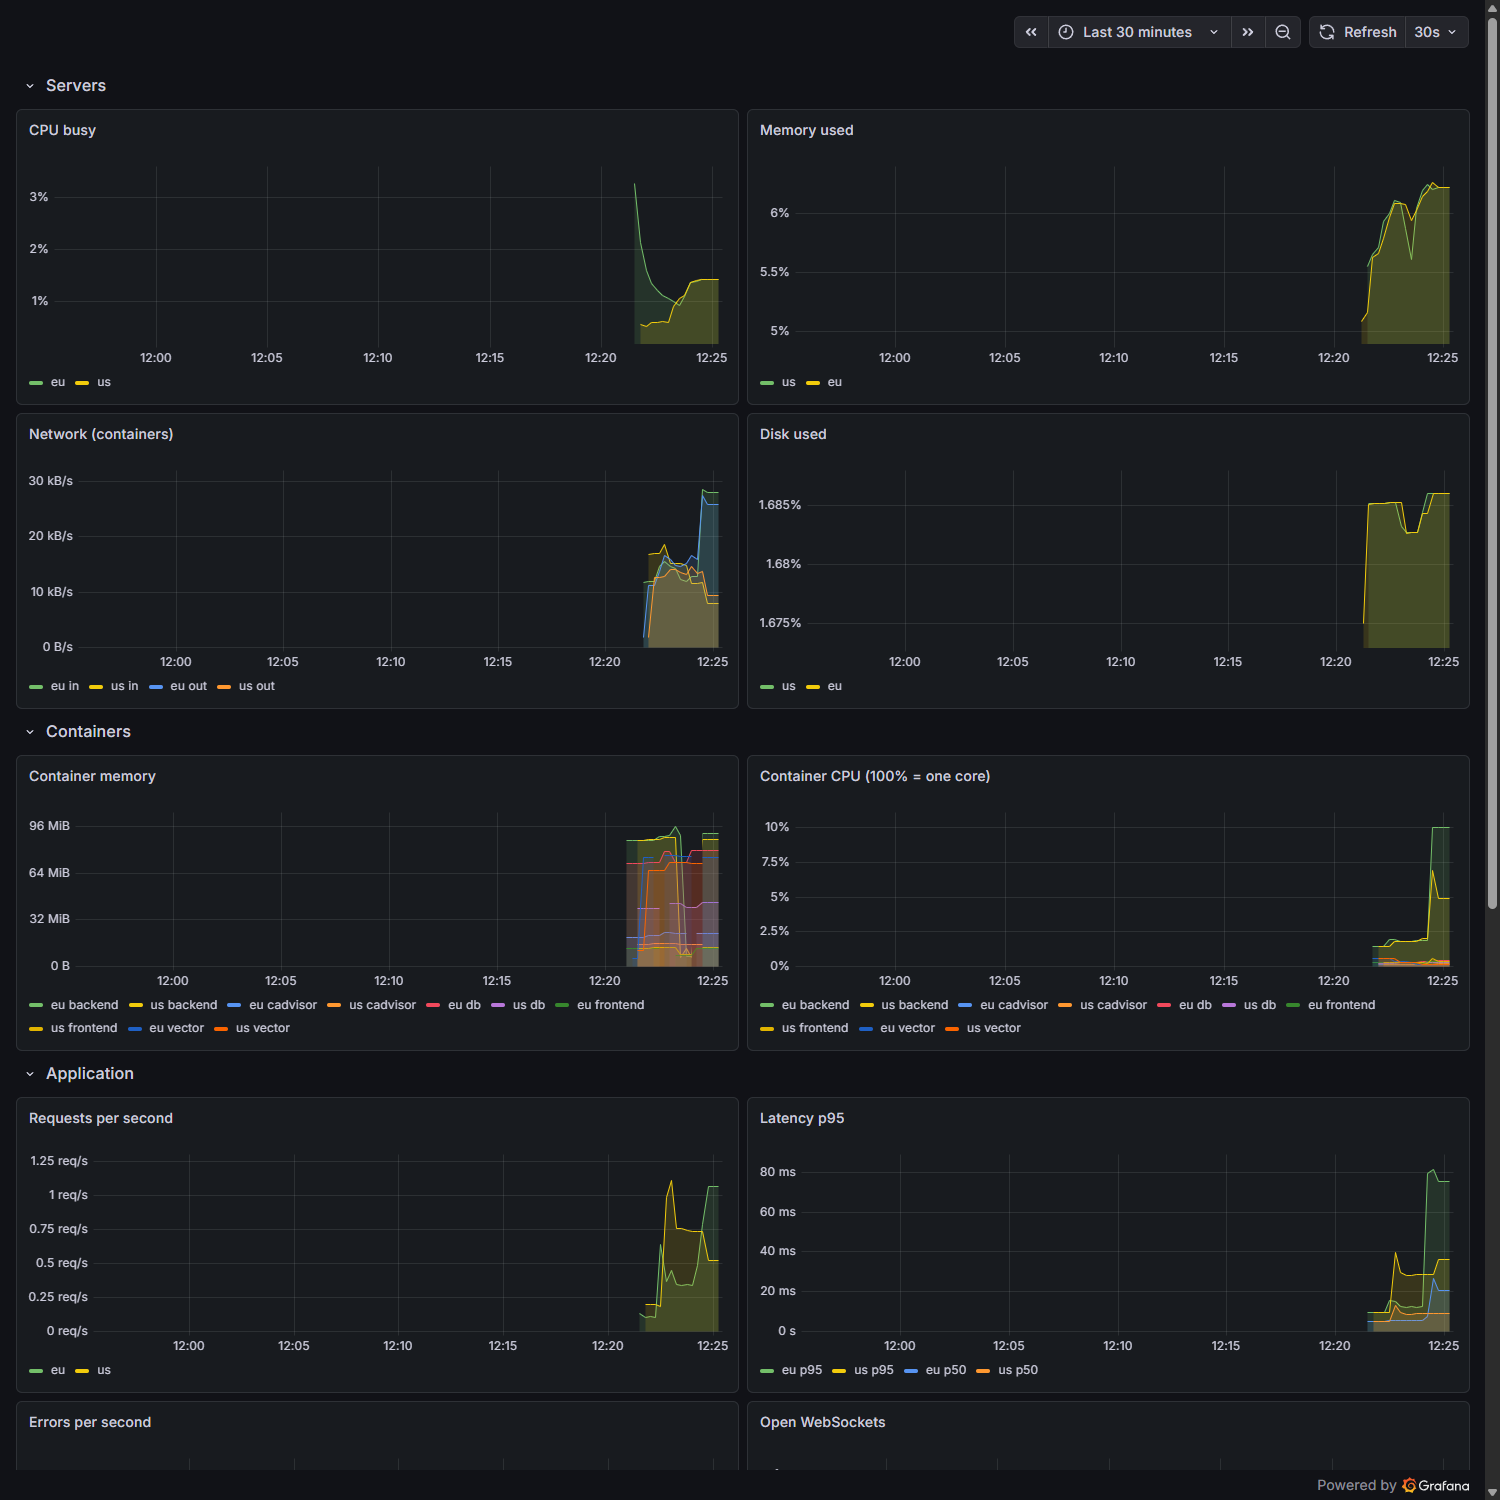
\includegraphics[width=0.95\textwidth]{obrazy/04-grafana.png}
\caption{Dashboard „PlayLink regions'': zasoby maszyn i kontenerów oraz ruch i opóźnienia obu regionów
(lokalny przebieg z ruchem eksperymentu F4).}
\end{figure}

Zużycie zasobów: region z agentami potrzebuje ok.\ 250~MB RAM, stos centralny ok.\ 350~MB, więc oba mieszczą się
na maszynie z 1~GB RAM i plikiem swap.

\subsection{Serwer MCP}
Serwer MCP (\code{backend/mcp_server}) działa lokalnie na komputerze użytkownika, tylko do odczytu, i łączy się
z publicznym API. Daje asystentowi AI narzędzia: \code{list_games}, \code{list_rooms}, \code{get_room_details},
\code{check_platform_health}, \code{search_logs} (LogsQL) i \code{query_metrics} (PromQL). Regiony są wykrywane
dynamicznie (\code{PLAYLINK_DOMAIN}, \code{PLAYLINK_REGIONS}). Sprawdzono działanie na produkcji w Azure:
\code{check_platform_health} zwrócił oba regiony jako dostępne (opóźnienie z laptopa przez Cloudflare ok.\
127~ms dla EU i 176~ms dla US), \code{search_logs} zwrócił świeże logi z maszyn, a \code{query_metrics} wykonał zapytanie bez błędu.
Instrukcja podłączenia dla Windows, macOS i Linuksa jest w \code{README.md}.

\fig{../diagrams/mcp.png}{0.95}{Serwer MCP: lokalnie albo na produkcji.}

% =====================================================================
\section{Wdrożenie na Azure}
\begin{table}[H]
\centering\footnotesize
\begin{tabularx}{\textwidth}{@{}llYY@{}}
\toprule
\textbf{Maszyna} & \textbf{Lokalizacja} & \textbf{Rola} & \textbf{Adresy} \\
\midrule
\code{playlink-eu} & \code{polandcentral} & Region EU & \code{playlink.<domena>}, \code{playlink-eu-api.<domena>} \\
\code{playlink-us} & \code{denmarkeast} & Region „US'' & \code{playlink-us.<domena>}, \code{playlink-us-api.<domena>} \\
\code{playlink-ops} & \code{polandcentral} & Logi, metryki, Grafana & \code{playlink-grafana}, \code{-logs}, \code{-metrics} \\
\bottomrule
\end{tabularx}
\caption{Maszyny \code{Standard_B2ats_v2} (2~vCPU, 1~GB RAM), Ubuntu 24.04, bez otwartych portów.}
\end{table}
Obsługa codzienna (\code{deploy/azure.sh start|stop|status|logs}) pozwala włączać maszyny tylko na czas prób.
Dane przetrwają zatrzymanie, bo baza leży na dysku systemowym. Maszyny są włączane tylko na czas prób
i pokazów, żeby oszczędzać kredyt studencki.

% =====================================================================
\section{Backlog zrealizowanych zadań}
\begin{table}[H]
\centering\footnotesize
\begin{tabularx}{\textwidth}{@{}lYl@{}}
\toprule
\textbf{Nr} & \textbf{Zakres} & \textbf{Filar} \\
\midrule
PR 91 & Wdrożenie wieloregionowe EU/US z Cloudflare Tunnel, wydania GHCR, aktualizacja pull-based, runbook & F1, F3 \\
PR 92 & Lokalny start EU/US, propozycja Stay/Switch, eksperyment obciążeniowy & F2, F4 \\
PR 96 & Serwer MCP (tylko odczyt) & F7 \\
PR 97 & Dynamiczne wykrywanie regionów w MCP & F7 \\
PR 99, issue 94 & Logi, metryki i Grafana, błędy frontendu, narzędzia logów w MCP, maszyna ops, Cloudflare Access & F7 \\
PR 101 & Źródło LaTeX dokumentu wizji w repozytorium & dokumentacja \\
PR 102 & Instrukcja podłączenia MCP do produkcji (Windows, macOS, Linux) & dokumentacja \\
Issue 95 & Implementacja Model Context Protocol & F7 \\
Issue 103 & Ten raport, diagramy, prezentacja i aktualizacja dokumentacji & dokumentacja \\
\bottomrule
\end{tabularx}
\end{table}

% =====================================================================
\section{Jakość i testy}
Zmiany przechodzą CI: lint backendu i frontendu, testy (po PR 99: 159 testów backendu i 69 frontendu),
walidacja migracji w PostgreSQL, walidacja plików compose i budowanie obrazów. Przed scaleniem PR 99 wykonano
niezależny przegląd kodu, a jego uwagi naniesiono. Wydania budują się dopiero po przejściu tych samych testów.

% =====================================================================
\section{Wnioski}
\begin{itemize}
  \item Dwa regiony da się stawiać i aktualizować jednym poleceniem i bez ręcznej pracy na maszynach; wystarczy
        do tego model pull-based i Cloudflare Tunnel, bez płatnych usług routingu.
  \item Maszyny nie mają otwartych portów: ruch wchodzi tunelem, a logi i metryki są wysyłane przez agentów.
  \item Lobby jest regionalne (pokoje nie są replikowane), co upraszcza system kosztem podziału społeczności graczy.
  \item Obserwowalność (logi, metryki, Grafana) mieści się na maszynach z 1~GB RAM, a serwer MCP daje asystentowi
        AI wgląd w pokoje, logi i metryki produkcji.
  \item Region „US'' stoi w Danii (\code{denmarkeast}), bo Azure for Students nie ma regionów w USA.
\end{itemize}

\section*{Załącznik: uruchomienie}
\begin{itemize}
  \item Lokalnie: \code{bash scripts/local-up.sh --both} (chooser \code{http://127.0.0.1:3000}).
  \item Azure: \code{bash deploy/azure.sh start|stop|status}.
  \item Logi i metryki lokalnie: \code{bash deploy/observability.sh up} (Grafana \code{http://127.0.0.1:3300}).
  \item MCP: sekcja „Model Context Protocol'' w \code{README.md}.
\end{itemize}

\end{document}
